\documentclass{standalone}

\usepackage{graphicx}
\usepackage{tikz}
\usetikzlibrary{arrows}
\usetikzlibrary{decorations.markings}

\begin{document}

\begin{tikzpicture}
  \node at (0, 0) {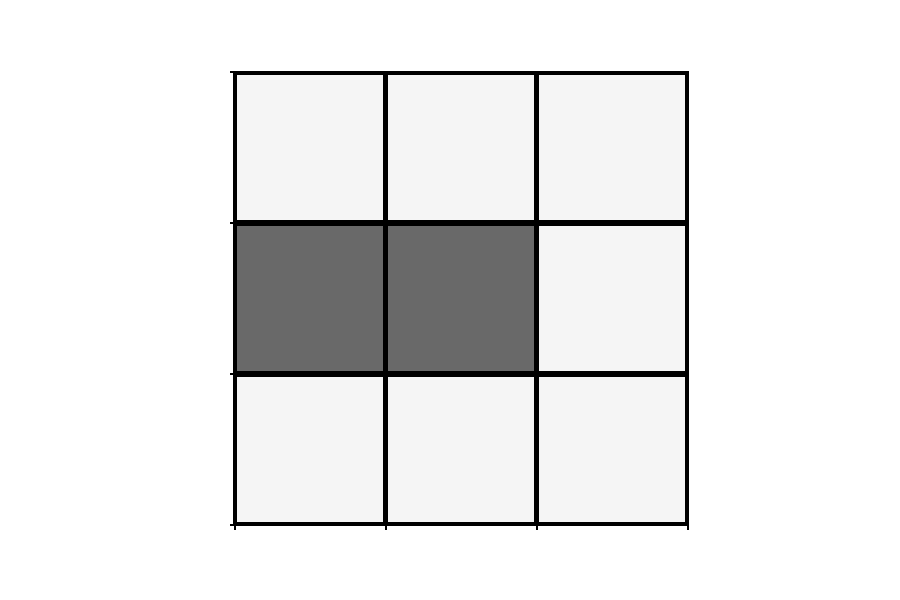
\includegraphics{init_1}};
  \draw[ultra thick, -triangle 90] (0, -5) -- (0, -6.5);
  \node at (0, -12) {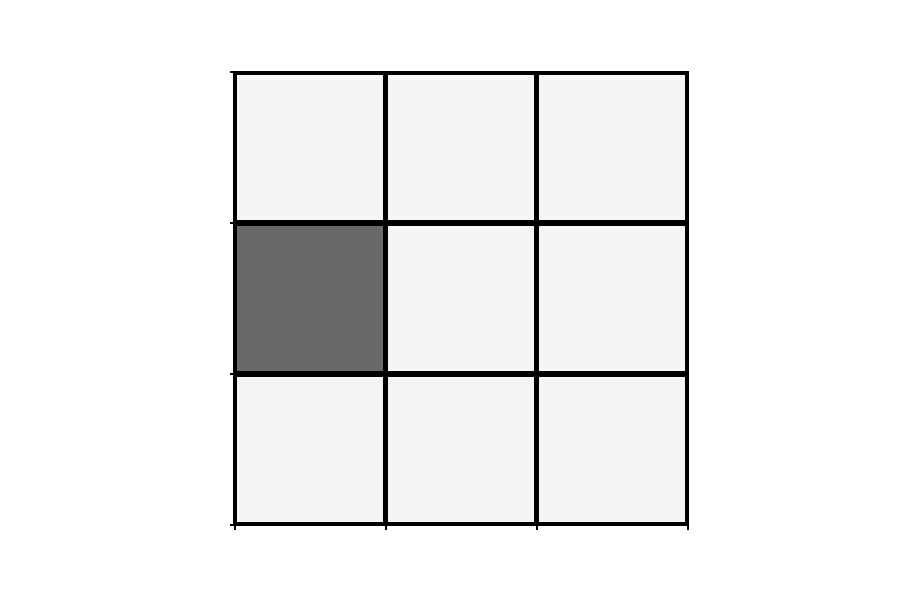
\includegraphics{after_1}};

  \node at (12, 0) {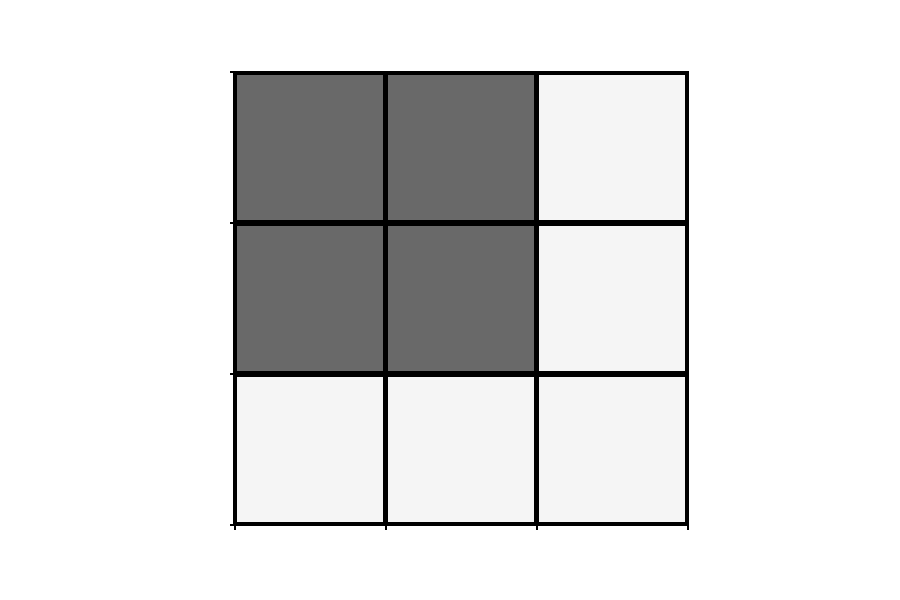
\includegraphics{init_2}};
  \draw[ultra thick, -triangle 90] (12, -5) -- (12, -6.5);
  \node at (12, -12) {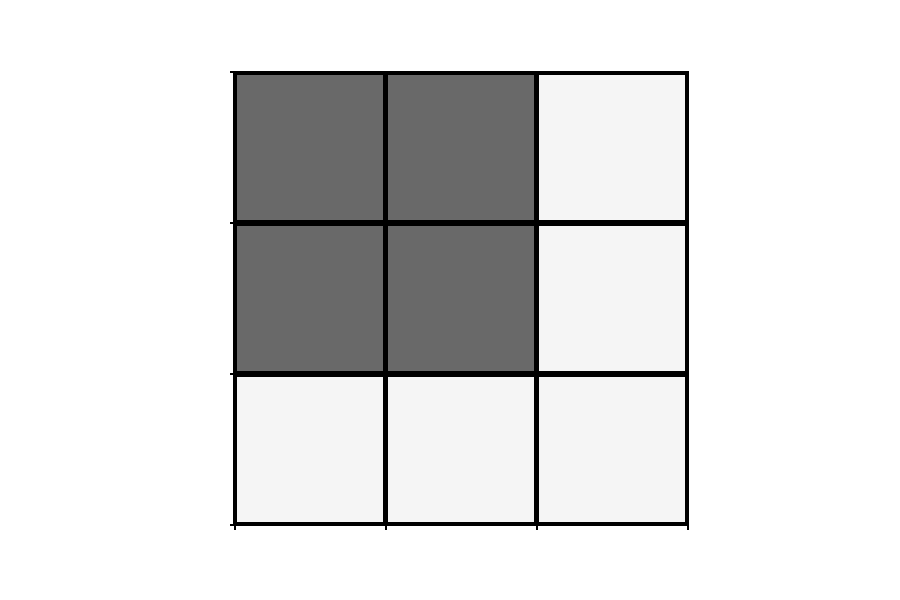
\includegraphics{after_2}};

  \node at (24, 0) {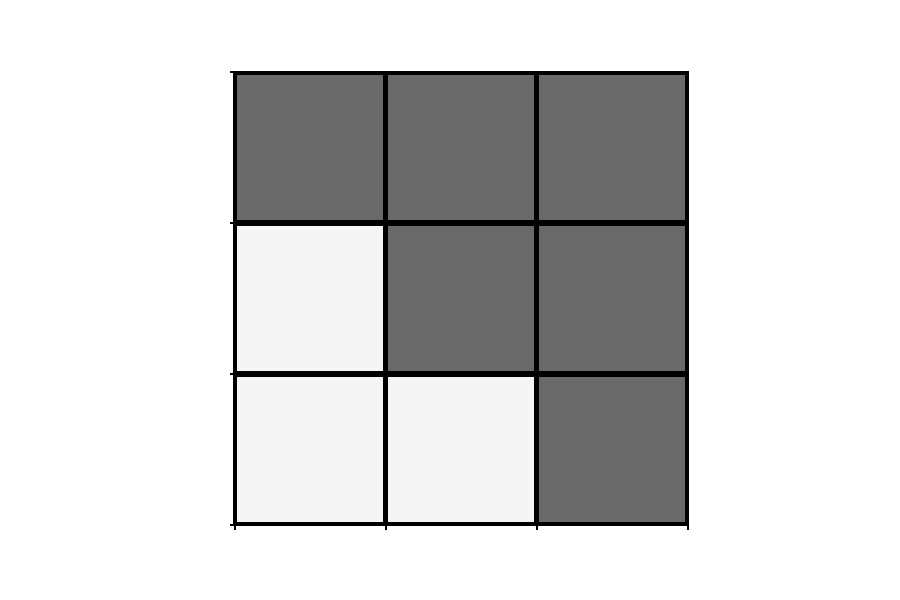
\includegraphics{init_3}};
  \draw[ultra thick, -triangle 90] (24, -5) -- (24, -6.5);
  \node at (24, -12) {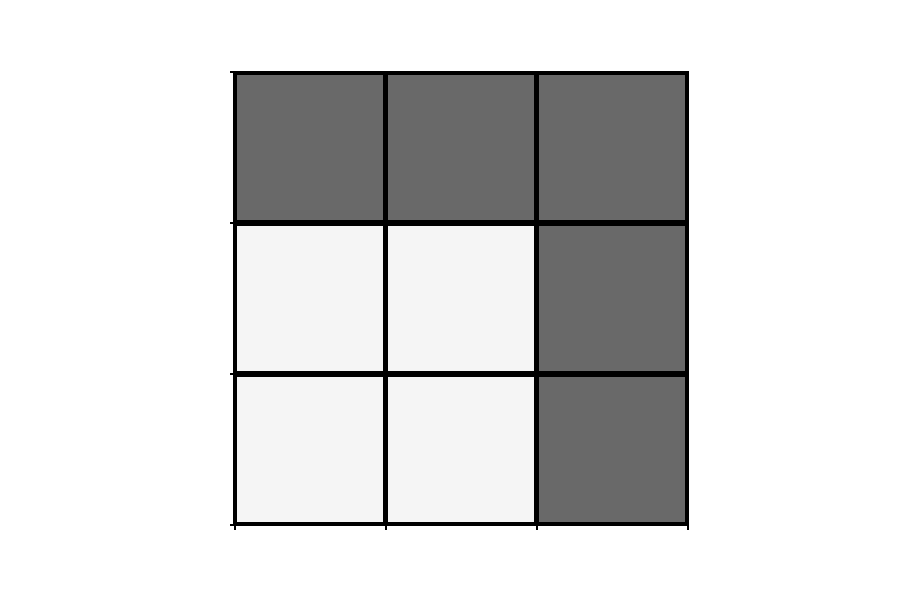
\includegraphics{after_3}};

  \node at (36, 0) {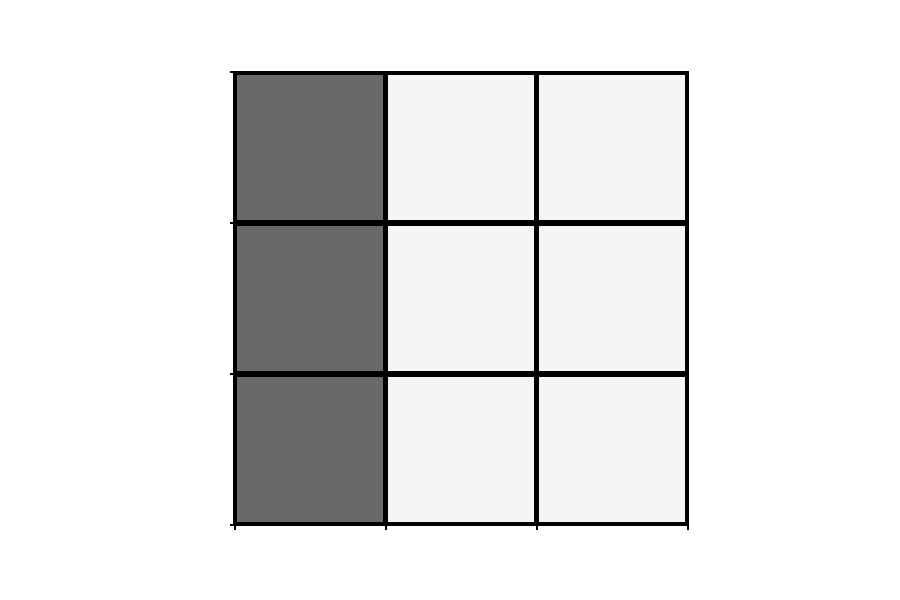
\includegraphics{init_4}};
  \draw[ultra thick, -triangle 90] (36, -5) -- (36, -6.5);
  \node at (36, -12) {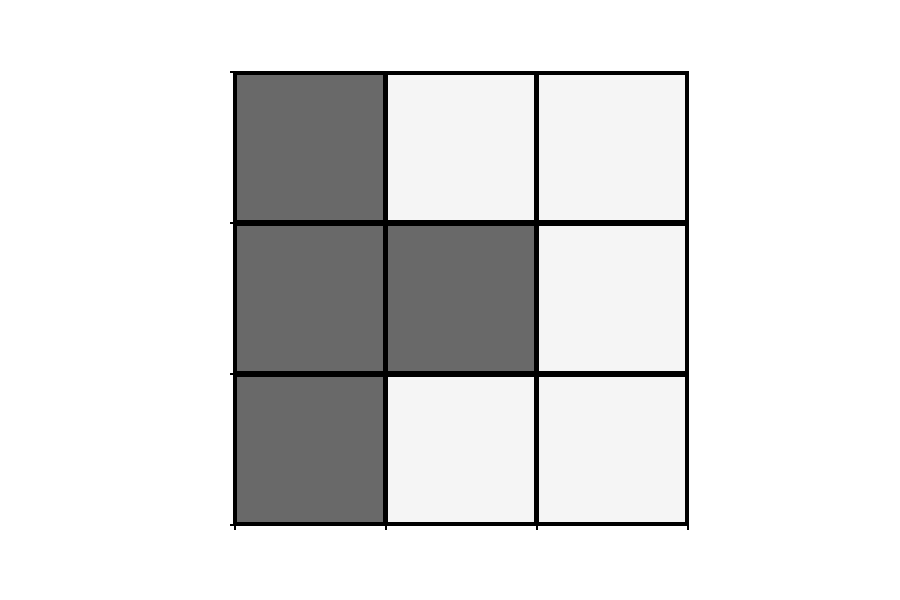
\includegraphics{after_4}};
\end{tikzpicture}

\end{document}
